\documentclass{beamer}
\usepackage[size=custom, width=121.9, height=91.44, scale=1.5, debug]{beamerposter} 
%\usepackage[size=custom, width=48in, height=36in, scale=1.4, debug]{beamerposter} 

\usetheme{Lankton}

\usepackage{amsmath, amsthm, amssymb, latexsym}
\usepackage[utf8]{inputenc}
\usepackage[T1]{fontenc}
\usepackage{mathpazo}
\usepackage[scaled=0.95]{berasans}
\usepackage[english]{babel}
\usepackage{graphicx}
\usepackage{float}
\usepackage{caption}

\graphicspath{{img/}}

\title{Ice retreat timing and bedrock erosion of the Puget Lobe of the Cordilleran ice sheet}
\newcommand{\footleft}{depts.washington.edu/cosmolab}
\newcommand{\footright}{zploskey@uw.edu}
\author{Zach Ploskey and John Stone}
\institute{Cosmogenic Nuclide Lab, Dept. of Earth and Space Sciences, University of Washington, Seattle}
\date{Aug. 8th, 2014}

\begin{document}

\begin{frame}{}\centering

\begin{columns}[T]

\begin{column}{0.32\columnwidth}

\begin{block}{Overview}	
During the Frasier glaciation, ice from the Cordilleran ice sheet flowed south from Canada across the San Juan Islands and into the Puget Lowland.
This ice lobe, known as the Puget Lobe, reached its maximum extent in the Puget Lowland 16.95 cal. ka ago  (Porter and Swanson, 1998), and soon after began to retreat.

\begin{figure}
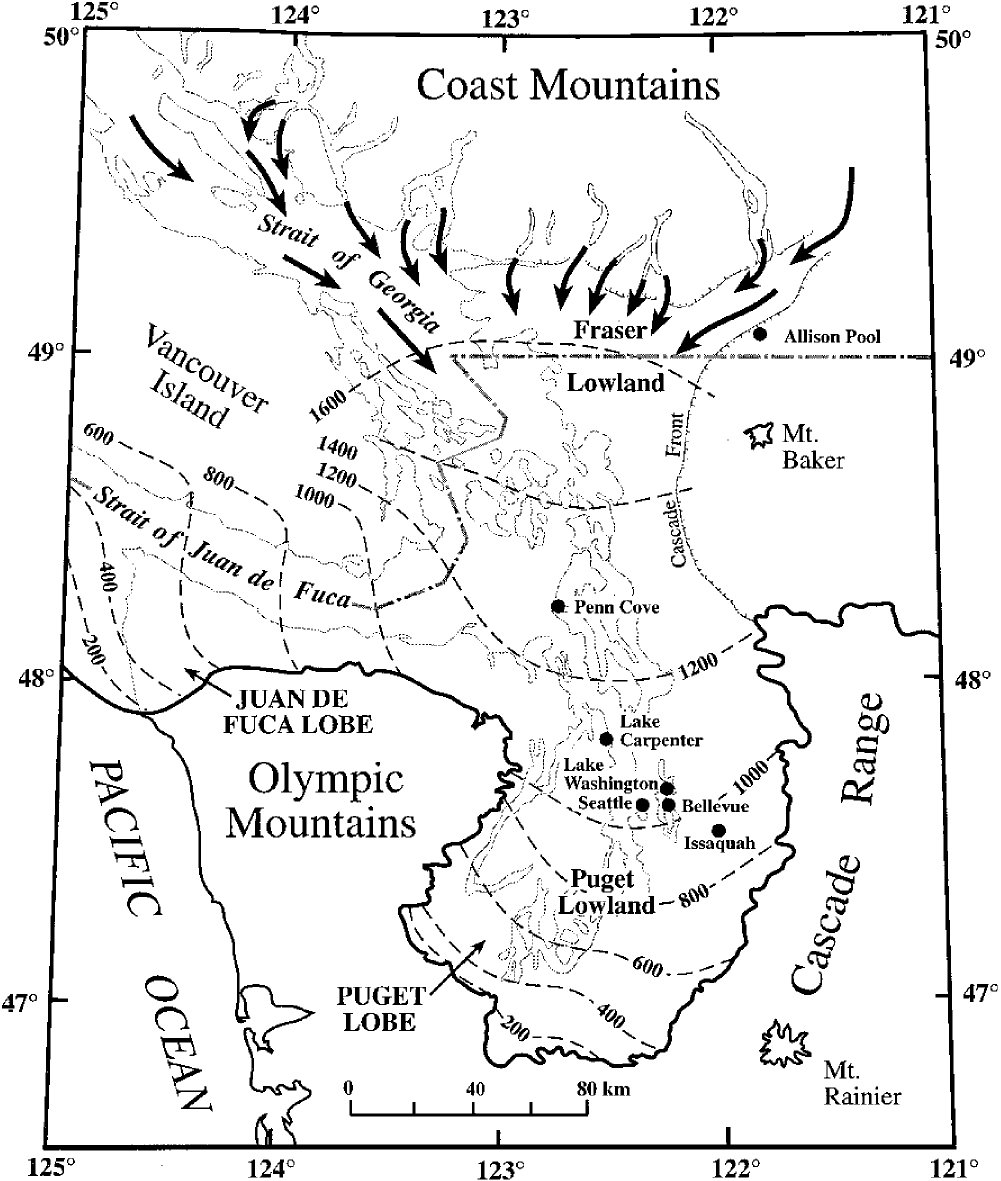
\includegraphics[width=0.5\textwidth]{lobe_map.png}
\caption*{Puget Lobe maximum extent (Porter and Swanson, 1998).}
\end{figure}

\end{block}

\begin{block}{Methods}
\begin{itemize}
\item We collected and measured cosmic ray-produced $^{10}$Be in glacial erratics and glacially eroded bedrock samples from the Puget Lowland and the San Juan Islands.
\item Measured $^{10}$Be concentrations in these rocks can be used to calculate exposure ages, and in the case of bedrock samples, infer the extent of erosion by glacial ice.
\item We compare the $^{10}$Be chronology to existing $^{14}$C dates from the Puget Lowland (Porter and Swanson, 1998).
\item Where dates diverge significantly from existing $^{14}$C chronology we can identify instances of limited erosion, resulting in anomalously high concentrations and apparent exposure ages, and shielding due to soil, sediment or tree cover, which diminishes the $^{10}$Be and apparent exposure age.
\end{itemize}
\end{block}

\end{column}
	
\begin{column}{.32\columnwidth}
	
\begin{block}{Goose Rock}

Bedrock samples from Goose  Rock, located on the north end of Whidbey Island, yielded apparent exposure ages older than downstream radiocarbon dates, which would require limited glacial erosion of the landform during the last glaciation.
Two overprinted sets of glacial striations preserved at Goose Rock may be related to a brief readvance of the retreating ice when it became grounded at Penn Cove, central Whidbey Island, following calving retreat.
Further exposure dating of erratic boulders or radiocarbon dates from Penn Cove are needed to test this hypothesis. 
	
\end{block}
	
\begin{block}{Mt. Constitution}
	
Bedrock samples collected further north, on Mt. Constitution, eastern Orcas Island, showed no prior exposure in a 5-sample north-south transect across the mountain and are consistent with radiocarbon ages located upstream and downstream of that location.
Exposure ages are consistent with an ice-free Mt. Constitution by ~14.5 ka. 

\end{block}

\end{column}

\begin{column}{.32\columnwidth}

\begin{block}{South Sound forest shielding}
\begin{itemize}
\item Large glacial erratic boulders in the southern Puget Lowland, near the ice sheet terminus, greatly underestimate the true exposure age, possibly due to heavy shielding from cosmic radiation in thick forest (Bretz 1913).
\item With independent age constraints, cosmogenic isotope measurements from these samples could be used to estimate forest canopy biomass following deglaciation.
\item Samples from southern Puget Sound near Olympia have apparent exposure ages that underestimate the true deglaciation age by 8\%, which is comparable to the $7\pm2\%$ shielding factor calculated for dense Olympia forest by Plug et al. (2007).
\end{itemize}
\end{block}

\begin{block}{Conclusions}
\begin{itemize}
\item Shielding of south Sound samples is consistent with forest comparable to the Olympic rainforest at the samples sites prior to western settlement.
\item Ice retreated north of the San Juan islands by 14.5 ka.
\item Exposure of bedrock at Goose Rock, northern Whidbey Island, has not been significantly eroded for at least two interglacial periods.
\end{itemize}
\end{block}

\begin{block}{References} 
{\small

\begin{itemize}


\item Bretz, J. H., 1913. Glaciation of the Puget Sound Region. Washington Geological Survey Bulletin 8, 244 pp.

\item Porter, S. C., Swanson, T. W., 1998. Radiocarbon Age Constraints on Rates of Advance and Retreat of the Puget Lobe of the Cordilleran Ice Sheet during the Last Glaciation. Quaternary Research 50, 205-213.

\item Plug, L. J., Gosse, J. C., McIntosh, J. J., Bigley, R., 2007. Attenuation of cosmic ray flux in temperate forest. Journal of Geophysical Research 112, F02022.

\end{itemize}

} %small
\end{block}

\begin{block}{Code}
	\center \url{github.com/zploskey/puget_lobe_amqua_2014_poster} 
	
\end{block}

\end{column}

\end{columns}

\end{frame}

\end{document}